% reset page numbers
\pagenumbering{arabic}
\setcounter{page}{1}

%%%%%%%%%%%%%%%%%%%%%%%%%%%%%%%%%%%%
% Title Page for Appendix
%%%%%%%%%%%%%%%%%%%%%%%%%%%%%%%%%%%%
% special footnote symbols
\renewcommand*{\thefootnote}{\fnsymbol{footnote}}
\begingroup
  \doublespacing
  \centering
  \Large ONLINE APPENDIX \\[1.5em]
  \LARGE \PAPERTITLE \\[0.75em]
  \large
    Fan Wang,\footnote[1]{\AUTHORWANG}\\[1.0em]
\endgroup
\clearpage

%%%%%%%%%%%%%%%%%%%%%%%%%%%%%%%%%%%%
% Appendix A, Solution and Estimation Details
%%%%%%%%%%%%%%%%%%%%%%%%%%%%%%%%%%%%

% Set equation, figure, table indexing
\renewcommand{\thefigure}{A.\arabic{figure}}
\setcounter{figure}{0}
\renewcommand{\thetable}{A.\arabic{table}}
\setcounter{table}{0}
\renewcommand{\theequation}{A.\arabic{equation}}
\setcounter{equation}{0}
\renewcommand{\thefootnote}{A.\arabic{footnote}}
\setcounter{footnote}{0}

\section{Solution and Estimation Details (Online Publication)}

\subsection{Reference Point and Preference for Height \label{sec:apprefsd}}

\subsubsection{The Optimal Nutritional-Choice Problem\label{sec:fullproblem}}
Given Equation \eqref{eq:budget_constraint} for the budget constraint, Equation \eqref{eq:prod_function} for the production function, Equation \eqref{eq:preferences} for preferences, and the reference points distributions discussed in Section \ref{sec:information}, the nutritional-choice problem is:
\begin{align}
    \begin{gathered}\label{eq:optimization}
        \max_{N}
        \left\{
            C + \rho\cdot C^{2} +
            \gamma \cdot H^{24} +
            \lambda \cdot \int_{R_{yv}} \left(H^{24}-R_{yv}\right)\mathbbm{1}\left\{ H^{24}\ge R_{yv}\right\}dF(R_{yv})
        \right\}
        \\
        C + p^{N}_{yv}\cdot(1-\delta\cdot\mathbbm{1}\left(v=Atole\right))\cdot N = Y\\
        H^{24} = \exp(A+ X\cdot\alpha+\epsilon)\cdot N^{\beta}
    \end{gathered}
\end{align}
For notational convenience, we drop subscripts, let $\hat{A}=\exp\left(A + X\cdot\alpha + \epsilon\right)$, replace $H^{24}$ and $C$ as functions of $N$, and rewrite Equation \eqref{eq:optimization} as:
\begin{align}
    \begin{gathered}\label{eq:optimization:single}
        \max_{N}
        \left\{
        \begin{array}{c}
            \left(Y - p \cdot N\right) +
            \rho\cdot\left(Y - p \cdot N\right)^{2} \\
            + \gamma \cdot \hat{A} \cdot N^{\beta} \\
            + \lambda \cdot \left(\hat{A} \cdot N^{\beta}-\mu_R\right)
                    \Phi\left(\frac{\hat{A} \cdot N^{\beta}-\mu_R}{\sigma_R}
                \right) \\
            + \lambda \cdot \sigma_R \cdot \phi\left(
                \frac{\hat{A} \cdot N^{\beta}-\mu_R}{\sigma_R}
                \right) \\
        \end{array}
        \right\}
    \end{gathered}
\end{align}
In Equation \eqref{eq:optimization:single}, we analytically integrate the integral from Equation \eqref{eq:optimization}.\footnote{The expected utility function contained the expectation of a truncated normal random variable:
\begin{multline}
	\int_{R_{yv}} \left(H^{24}-R_{yv}\right)\mathbbm{1}\left\{ H^{24}\ge R_{yv}\right\}dF(R_{yv})=  \left(H^{24}-\mu_{R_{yv}}\right)\cdot\left(\Phi\left(\frac{H^{24}-\mu_{R_{yv}}}{\sigma_{R_{yv}}}\right)\right)+\sigma_{R_{yv}}\phi\left(\frac{H^{24}-\mu_{R_{yv}}}{\sigma_{R_{yv}}}\right) \label{eq:truncatedNormal}
\end{multline}}

\subsubsection{Optimal Nutritional Choices and $\sigma_R$\label{sec:sigmaopti}}

Panels a, c, and e of Figure \ref{fig:refpointhgtutil} show health (height) at age 24 months along the x-axis and household consumption along the y-axis. We plot the shape of indifference curves for a given value of $\gamma$ and different values of $\lambda$ and $\sigma_R$ together with the consumption-health possibility frontier, which combines the budget constraint with the production function for height.

Panels b, d, and f show the difference between height at age 24 months and the mean beliefs about the reference height along the x-axis, and the component of utility that  includes the reference point for height along the y-axis. We believe it is helpful to zero in on this component because it is the primary driver of our empirical analysis, and it shows the role that the parameters $\lambda$ and $\sigma_R$ play in our study of the determinants of height at age 24 months.

In panels a and b, we use our estimated values of $\gamma$ and $\lambda$ for the scenario in which $\sigma_R = 0.5$. In panels c and d, we set $\lambda$ to be negative $1.5$ times the estimated value of $\gamma$. In panels e and f, the $\lambda$ value is lowered to be negative $2.5$ times the estimated value of $\gamma$.

For the configuration of values of $\gamma$ and $\lambda$ in panel a, an increase in $\sigma_R$ increases optimal height because the marginal benefits of height levels that exceed $\mu_{R}$ remains positive as panel b shows. However, for the configuration of values of $\gamma$ and $\lambda$ in panel c, we have a bliss point for height that varies just a little as we increase the value of $\sigma_R$. In panel e, as the value of $\lambda$ continues to decrease, the disutility of height beyond the mean reference point decreases so fast that the uncertainty becomes costly. As a result, an exogenous increase in $\sigma_R$ reduces the optimal level of height.

\newcommand{\subFigWidthApp}{0.50}
\begin{figure}[hbt!]
    \centering
    \begin{subfigure}[b]{\subFigWidthApp\textwidth}
        \centering
        \includegraphics[width=\linewidth]{\string"fig_main/fig1d_Tester_Indiff_person_495_refsd_increasem3_20210130".eps}
        \caption{Choices with $\gamma=0.0325$, $\lambda=-0.0257$}
    \end{subfigure}~
	\begin{subfigure}[b]{\subFigWidthApp\textwidth}
	    \centering
    	\includegraphics[width=\linewidth]{\string"tab_fig_online_appendix/fig_a1b_Tester_UHgt_moresd_higherH".eps}
    	\caption{Health preference with $\gamma=0.0325$, $\lambda=-0.0257$}
	\end{subfigure}
	\par\medskip
	\begin{subfigure}[b]{\subFigWidthApp\textwidth}
        \centering
        \includegraphics[width=\linewidth]{\string"tab_fig_online_appendix/fig_a1c_Tester_Indiff_person_495_refsd_noimpactm3_20210130".eps}
        \caption{Choices with $\gamma=0.0325$, $\lambda=-\gamma\cdot1.5$}
    \end{subfigure}~
	\begin{subfigure}[b]{\subFigWidthApp\textwidth}
	    \centering
	    \includegraphics[width=\linewidth]{\string"tab_fig_online_appendix/fig_a1d_Tester_UHgt_moresd_noimpact".eps}
	    \caption{Health preference with $\gamma=0.0325$, $\lambda=-\gamma\cdot1.5$}
	\end{subfigure}
	\par\medskip
	\begin{subfigure}[b]{\subFigWidthApp\textwidth}
        \centering
        \includegraphics[width=\linewidth]{\string"tab_fig_online_appendix/fig_a1e_Tester_Indiff_person_495_refsd_decreasem3_20210130".eps}
        \caption{Choices with $\gamma=0.0325$, $\lambda=-\gamma\cdot2.5$}
    \end{subfigure}~
	\begin{subfigure}[b]{\subFigWidthApp\textwidth}
	    \centering
	    \includegraphics[width=\linewidth]{\string"tab_fig_online_appendix/fig_a1f_Tester_UHgt_moresd_lowerH".eps}
	    \caption{Health preference with $\gamma=0.0325$, $\lambda=-\gamma\cdot2.5$}
	\end{subfigure}
	\caption{Reference points distribution standard deviation ($\sigma_R$) and health outcomes}
	\label{fig:refpointhgtutil}
\end{figure}
\pagebreak

\clearpage
\pagebreak

\subsection{Alternative Assumptions about Variance Beliefs} \label{sec:appsecalter}

Our model assumes that parents adopt the expected height of two-year-old children in their village as the reference point. Parents estimate the expected height using the observations of the children in their village. We assume that their estimation of the expected height follows a normal distribution with mean belief parameter $\mu_{R_{y,v}}$ and variance belief parameter $\sigma_{R{y,v}}^{2}$. In our empirical analysis, we assume that $\mu_{R_{y,v}}$  captures the uncertainty about the mean belief, so  $\sigma_{R{y,v}} = 0.5$.

In our sensitivity analysis, we adopt the assumption that the variance belief is equal to the variance of height. We argue that this approach is an upper bound for variance beliefs. Under this assumption, $\sigma_{R{y,v}} = 3.5$. To complete our sensitivity analysis, we also investigate our model's decomposition findings for scenarios in which $\sigma_{R{y,v}} = 1.5$ and $\sigma_{R{y,v}} = 2.5$.

\subsection{Data for Estimation \label{sec:estidata}}

We include in the estimation children who were born between 1970 and 1975. We show summary statistics for these children in Sections \ref{sec:stat} and \ref{sec:gap}. As discussed earlier, we do not observe both initial heights and heights at month 24 for children born before or after these years.

We use the months 15 to 24 average protein intakes, heights at month 24, protein prices, incomes, gender, and initial height variables shown in Table \ref{summcovarmain} and described in Section \ref{sec:stat} as $N$, $H^{24}$, $p_{yv}^{N}$, $Y$, and components of $X$. We use protein intakes because \textcite{puentes_early_2016} shows that proteins rather than non-protein components of calories matter for height growth in these INCAP data. Ideally, our intake variable should be averaged from month 0 to month 24. However, we do not observe protein values from month 0 to month 12 for close to half of our sample because data collection for this age group started in 1973. Also, it is not easy to estimate the protein component of breastmilk for children who rely on breastfeeding in the first year of life.

\subsection{Additional Estimation Information \label{sec:estimorer}}

\subsubsection{Additional Model fit}
\begin{table}[htbp]
\renewcommand{\arraystretch}{1.3}
\centering
{\small
\def\sym#1{\ifmmode^{#1}\else\(^{#1}\)\fi}
\caption{Model Predictions from estimating the model under different assumptions about the standard deviation of reference points distribution $\sigma_{R}$.\label{tab:paramfitmulti}}
\begin{adjustbox}{max width=1\textwidth}
\begin{tabular}{lcccc|cccc}
\toprule
& \multicolumn{4}{C{6cm}}{\hspace*{-10mm}\textbf{Average protein choices}} & \multicolumn{4}{C{6cm}}{\hspace*{-15mm}\textbf{Average height outcome}} \\
\cmidrule(l{5pt}r{5pt}){2-5} \cmidrule(l{5pt}r{5pt}){6-9}
& \multicolumn{1}{C{1.5cm}}{\textit{\small$\sigma_R=0.5$}} & \multicolumn{1}{C{1.5cm}}{\textit{\small$\sigma_R=1.5$}} & \multicolumn{1}{C{1.5cm}}{\textit{\small$\sigma_R=2.5$}} & \multicolumn{1}{C{1.5cm}}{\textit{\small$\sigma_R=3.5$}} & \multicolumn{1}{C{1.5cm}}{\textit{\small$\sigma_R=0.5$}} & \multicolumn{1}{C{1.5cm}}{\textit{\small$\sigma_R=1.5$}} & \multicolumn{1}{C{1.5cm}}{\textit{\small$\sigma_R=2.5$}} & \multicolumn{1}{C{1.5cm}}{\textit{\small$\sigma_R=3.5$}} \\      
\midrule
\multicolumn{9}{l}{\hspace*{0mm}\textbf{\normalsize Panel a: Average}} \\
Fresco          &  19.38&   19.24&   19.25&   19.29&   76.77&   76.77&   76.78&   76.77\\
Atole           &  25.10&   25.30&   25.30&   25.47&   78.19&   78.32&   78.33&   78.39\\
\midrule
\multicolumn{9}{l}{\hspace*{0mm}\textbf{\normalsize Panel b: Averages across genders}} \\
Fresco Female   &  18.15&   18.14&   18.16&   18.15&   76.07&   76.11&   76.12&   76.11\\
Fresco Male     &  23.96&   24.17&   24.17&   24.24&   77.60&   77.74&   77.75&   77.81\\
Atole Female    &  20.48&   20.23&   20.23&   20.30&   77.40&   77.36&   77.36&   77.35\\
Atole Male      &  26.16&   26.34&   26.33&   26.60&   78.74&   78.85&   78.86&   78.93\\
\midrule
\multicolumn{9}{l}{\hspace*{0mm}\textbf{\normalsize Panel c: Averages across years}} \\
Fresco 1970-71  &  18.43&   18.61&   18.63&   18.61&   76.52&   76.59&   76.60&   76.57\\
Atole  1970-71  &  23.13&   23.52&   23.46&   23.46&   77.71&   77.85&   77.85&   77.88\\
Fresco 1972-73  &  19.30&   19.22&   19.24&   19.25&   76.80&   76.79&   76.79&   76.79\\
Atole  1972-73  &  24.51&   24.76&   24.76&   24.92&   78.07&   78.20&   78.20&   78.27\\
Fresco 1974-75  &  19.97&   19.61&   19.61&   19.69&   76.89&   76.86&   76.86&   76.85\\
Atole  1974-75  &  27.13&   27.13&   27.15&   27.46&   78.65&   78.78&   78.80&   78.87\\
\bottomrule
\addlinespace[0.5em]
\multicolumn{9}{p{1\textwidth}}{\parbox[t]{1\textwidth}{}}\\
\end{tabular}\end{adjustbox}
}
\end{table}






In Table \ref{tab:paramfitmulti}, we provide additional information on the fits of the estimated model under varying assumptions about $\sigma_{R_{y,v}}$. Model fits with respect to protein choices and height outcomes are presented across the columns, and model fits with respect to overall averages in Atole and Fresco villages, as well as average by gender and time are presented in separate rows.

Estimated models across $\sigma_{R_{y,v}}$ assumptions -- with estimates shown in Table \ref{tab:paramesti} -- are all able to provide similarly good fits between model predictions and key data moments.

\subsubsection{Additional Estimates}

\begin{figure}[htbp]
\makebox[\textwidth][c]{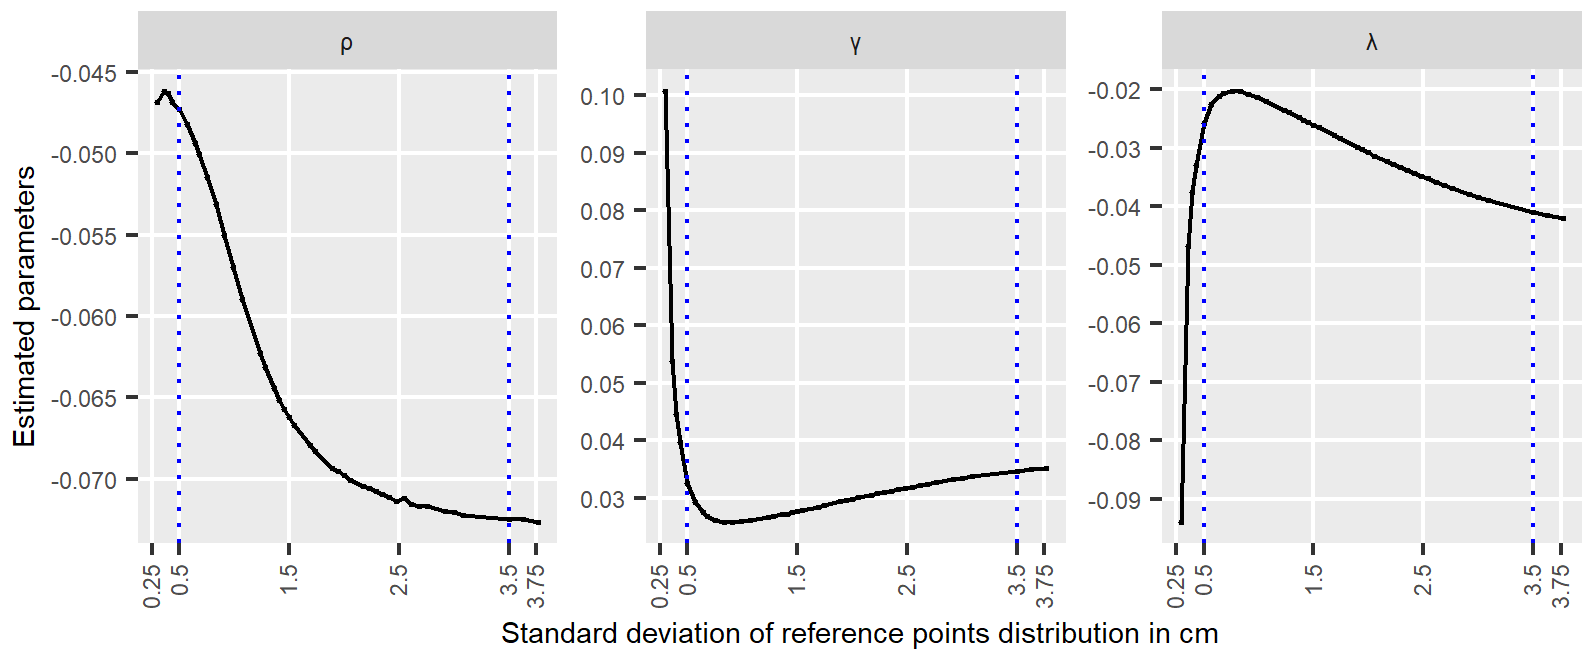
\includegraphics[width=1.10\textwidth]{tab_fig_online_appendix/fig_a2_estimates_final.png}}
\caption{Preference parameter estimates from estimating the model under different assumptions about the standard deviation of reference points distribution $\sigma_{R_{y,v}}$}
\label{fig:estimatesmulti}
\end{figure}

In Table \ref{tab:paramesti}, we present parameter estimates under four assumptions for $\sigma_{R_{y,v}}$ from 0.5 cm to 3.5 cm. In this section, for additional information, we provide key estimates from estimating the model at $\sigma_{R_{y,v}}$ values from 0.25 cm to 3.75 cm at 0.05 cm intervals. In Figure \ref{fig:estimatesmulti}, we visualize the point-estimates results for the core preference parameters of $\rho$, $\gamma$ and $\lambda$ in three sub-figures. We mark with dashed blue lines values of $\sigma_{R_{y,v}}$ along the x-axis where $\sigma_{R_{y,v}}=0.5$ and $\sigma_{R_{y,v}}=3.5$.

For $\rho$, the quadratic coefficient on non-nutritional consumptions, the estimated coefficient becomes more negative as $\sigma_{R_{y,v}}$ increases. This finding implies lower marginal gains from additional non-nutritional consumption at higher $\sigma_{R_{y,v}}$.

\clearpage
\pagebreak

%%%%%%%%%%%%%%%%%%%%%%%%%%%%%%%%%%%%
% Appendix Bibliography
%%%%%%%%%%%%%%%%%%%%%%%%%%%%%%%%%%%%

% Bibliography
\begingroup
\setstretch{1.0}
\setlength\bibitemsep{0pt}
\printbibliography[title=References for Online Appendix]
\endgroup
\pagebreak
